\section{Application to path tracing}
\label{sec::appli_pathtrace}

In this section, we explain how to use the curvilinear skeleton of the voids of the scene in order to enhance the path tracing algorithm. We start by defining some basic elements related to path tracing and we present our skeleton based path tracing algorithm.

%\subsection{Basic definitions of radiometry}
%
%Let $S$ be a set of surfaces of $\Rset^3$ that don't overlap and $S_L \subset S$ a set of surface lights. $S$ is called the scene.
%
%The basic radiometric quantity is the \myem{radiance} $L(x \rightarrow \Theta)$ that expresses the quantity of light energy produced by the surface point $x \in \Rset^3$ toward direction $\Theta \in \Omega_x$ per unit of time per unit area per unit solid angle (expressed in $W.m^{-2}.sr^{-1}$).
%This is the quantity that the eye actually "sees" and that must be computed for each pixel of the final image.
%
%% image radiance
%
%We can define another quantity related to radiance called \myem{incoming radiance} $L(x \leftarrow \Phi)$ that represents the radiance that reach $x$ from direction $\Phi$.
%
%In the void, incoming radiance can be written in terms of radiance as follow:
%
%\begin{equation*}
%L(x \leftarrow \Phi) = L(r(x, \Phi) \rightarrow -\Phi)
%\end{equation*}
%
%$r(x, \Phi)$ is the surface point seen by $x$ in the direction $\Phi$. It can be defined formally by:
%
%\begin{align*}
%r(x, \Phi) &= x + t_{min}\Phi \\
%t_{min} &= min \lbrace t \in (0, +\infty]~ |~ x + t\Phi \in S \rbrace
%\end{align*}
%
%If $t_{min} = \infty$ then $r(x, \Phi)$ is undefined and $L(x \leftarrow \Phi) = 0$. We call $r$ the \myem{raytrace} function. In practice it is implemented by throwing a ray in the scene and looking for the first intersection.
%
%A third quantity related to radiance is \myem{emitted radiance} $L_e(x \rightarrow \Theta)$. It is not null if $x$ is a point of a light source ($x \in S_L$). In practice the emitted radiance is given with the set $S_L$ as an input of the algorithm.
%
%The radiance is the solution of an equation called the Rendering Equation:
%
%\begin{align*}
%L(x \rightarrow \Theta) &= L_e(x \rightarrow \Theta) + \int_{\Phi \in \Omega_x} f_r(x, \Theta \leftrightarrow \Phi) L(x \leftarrow \Phi) cos(N_x, \Phi) d\omega_\Phi \\
%&= L_e(x \rightarrow \Theta) + L_r(x \rightarrow \Theta)
%\end{align*}
%
%This equation expresses an intuitive idea: the radiance produced by the point $x$ in the direction $\Theta$ is the sum of the emitted radiance and the reflected radiance.  The reflected radiance is computed by integrating the incoming radiance scaled by a factor $f_r(x, \Theta \leftrightarrow \Phi) cos(N_x, \Phi)$ over all the possible directions of the hemisphere around $x$. $N_x$ is the surface normal at point $x$.
%
%The $f_r$ function is called the \myem{bidirectional reflectance function} (BRDF) and express the exchange of radiance between the incoming direction $\Phi$ and the output direction $\Theta$. Intuitively it represents the material properties of the surface at point $x$. A mirror doesn't reflect light the same manners a wall do, the BRDF encodes that.
%
%It's actually the rendering equation that a path tracer try to resolve. Let $O$ be the origin of the camera and $I$ the image we want to compute (a rectangle embedded in $\Rset^3$). Then the path tracing algorithm compute an approximation of the radiances $L(O \leftarrow \vec{OP})$, $\forall P \in I$.

\subsection{The path tracing}

Let $O$ be the origin of the camera in the scene. For each pixel $P$ of the final image, let $x$ be the nearest intersection point of the ray $(O, \overrightarrow{OP} = -\Theta)$ with an element of the scene. To obtain the luminosity, we must solve the rendering equation \cite{Ka86} which is a recursive integral equation. The integrand of the equation contains the radiance function that we must compute:

\begin{align*}
L(x \rightarrow \Theta) &= L_e(x \rightarrow \Theta) + \int_{\Phi \in \Omega_x} f_s(x, \Theta \leftrightarrow \Phi) L(r(x, \Phi) \rightarrow -\Phi) d\omega_\Phi
\end{align*}

$L$ is the radiance (a radiometric quantity that represents luminosity) from point $x$ toward direction $\Theta$. $L_e$ is the emitted radiance (non null only on light sources). The point $r(x, \Phi)$ is the nearest visible point from $x$ in the direction $\Phi$ of the hemisphere $\Omega_x$. The $f_s$ function expresses how much luminosity is exchanged, on point $x$, between an incoming ray $\Phi$ and the outgoing ray $\Theta$. Intuitively it represents the material properties of the surface at point $x$.

This integrand expresses an intuitive idea: the reflected radiance from $x$ towards the camera is the result of computing all incoming luminosity on $x$ scaled by a factor which depends on the material on $x$ and the angle of the ray going from the camera to $x$. The most common method used to estimate the integral, denoted by $L_r(x \rightarrow \Theta)$, is the Monte-Carlo integration which provides the following:

\begin{equation*}
\langle L_r(x \rightarrow \Theta) \rangle = \frac{f_s(x, \Theta \leftrightarrow \Phi) L(r(x, \Phi) \rightarrow -\Phi)}{p(\Phi)}
\end{equation*}

where $p$ is a probability density function (pdf) that is used to sample $\Phi$. This estimator is unbiased, meaning that the expected value $E[\langle L_r(x \rightarrow \Theta) \rangle]$ is equal to $L_r(x \rightarrow \Theta)$. The variance of the estimator expresses its quality and depends on the choosen pdf $p$. The best choice is a pdf that matches the shape of the function to integrate (ie. give high density to samples that have high values for the function and low density to samples that have low values).
The strategy of choosing an adapted pdf is called \myem{importance sampling} and is used in global illumination to improve the convergence speed of the algorithms.

The algorithm computes $L$ as follow: first, it chooses one random direction $\Phi$ based on the pdf $p$. Then, it applies the estimator by calling $L$ recursively to compute $L_r$ (shoots a new ray in the direction $\Phi$, computes the new hit point with the scene, and compute the new radiance at this point). Finally, it returns the sum of the emitted radiance $L_e$ and the result for $L_r$. The recursion stops when a maximal number of bounces has been reached.
%ASK: euh, c'est L ou L_r%
%c'est bon de dire que �a s'arrete au light%

This computation is done multiple times for each pixel (at different positions over the pixel). We average the results and get an estimation of the mean radiance passing through the pixel and heading towards the camera.
%at different positions over the pixel  ???%
A bad pdf would lead in picking directions that don't reach the light before the end of the recursion, and produce results with a lot of noise in the final image. In the next part, we explain how to produce a pdf based on the curvilinear skeleton.



\subsection{Skeleton based importance sampling}

As stated in the introduction, a curvilinear skeleton of the void (with some preprocessing achieved on it) gives us information on which directions the light comes from. Given these directions, we can build a efficient pdf $p_{skel}$ and guide our rays by sampling the hemispheres with $p_{skel}$.

The integrand of $L_r$ is:

%a revoir, je ne comprends pas tout

\begin{equation*}
f_s(x, \Theta \leftrightarrow \Phi) L(r(x, \Phi) \rightarrow -\Phi).
\end{equation*}

It is a product of two functions that can be efficiently sampled individually but that are hard to sample when they are combined. The most common strategy used to sample $\Omega_x$ is to use the function $f_s$ because we know it: it is given as an input of the algorithm, for exemple with textures that describe materials.

The term $L$ is rarely used because its evaluation cannot be done in constant time. Remember that it represents the distribution of light in the scene. It takes high values when $\Phi$ carries a lot of energy. Our method gives a way to sample according to $L$.



\subsubsection{Construction of the importance points}

The skeleton of the voids of the scene is computed using Alg.~\ref{algo::3d_curvskel} and is converted to a graph (the nodes are the 0-faces and the edges are the 1-faces). We then compute a set of \myem{importance points}: these points will be used to sample $\Omega_x$ in the path tracing algorithm. For each node of the skeleton $n$, one importance point $imp_n$ is computed. Intuitively, the importance point associated to $n$ gives us a direction to follow in order to find a light source.
%TODO a verifier quand meme

%La, pas clair !!!
Let $L$ be a light source of the scene ($L \in S_L$) and $n_L$ the nearest node that is visible by $L$. We first compute a tree of shortest paths along the skeleton with $n_L$ as root. We use the Dijkstra algorithm with a distance based on visibility from $n_L$: We put $d(n, m) = 1$ if $m$ is visible from $n_L$ and $d(n, m) = 10$ if not. It results that the paths that are enlighted by $L$ will have a shorter distance and will guide us to the light faster than the dark ones.

Let $n$ be a node of the skeleton and $V_n$ the set of visible nodes from $n$ along the shortest path toward $n_L$. The importance point $imp_n$ associated to $n$ is the barycenter of $V_n$.

\begin{center}
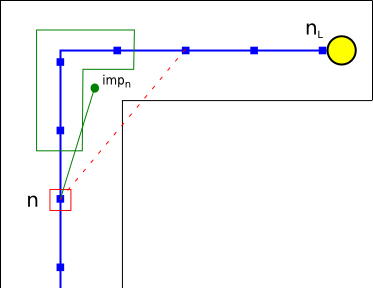
\includegraphics[scale=0.5]{images/importance_points.png}
\end{center}

\subsubsection{Sampling according to $L$}

Given a point $x$ and a direction $\Theta$ we want to compute $L(x \rightarrow \Theta)$ and then sample the hemisphere $\Omega_x$. We search for the nearest skeleton node $n$ and its importance point $imp_n$. We sample the hemisphere with a power-cosine pdf centered on $\overrightarrow{ximp_n}$:

\begin{equation*}
p_{skel}(\Phi) = \frac{s + 1}{2\pi} cos^s \alpha
\end{equation*}

with $\alpha$ the angle between $\overrightarrow{ximp_n}$ and $\Phi$, $s$ being a parameter called skeleton strength. The higher $s$ is, the more we sample close $\overrightarrow{ximp_n}$.

\subsection{Results and discussion}

We present some results of our algorithm applied to four scenes. The first row shows our result and the second row shows a standard path tracing with the same input parameters. On each picture a MSE (mean square error) value with a reference image is shown.

\begin{figure}[htp]
\begin{center}
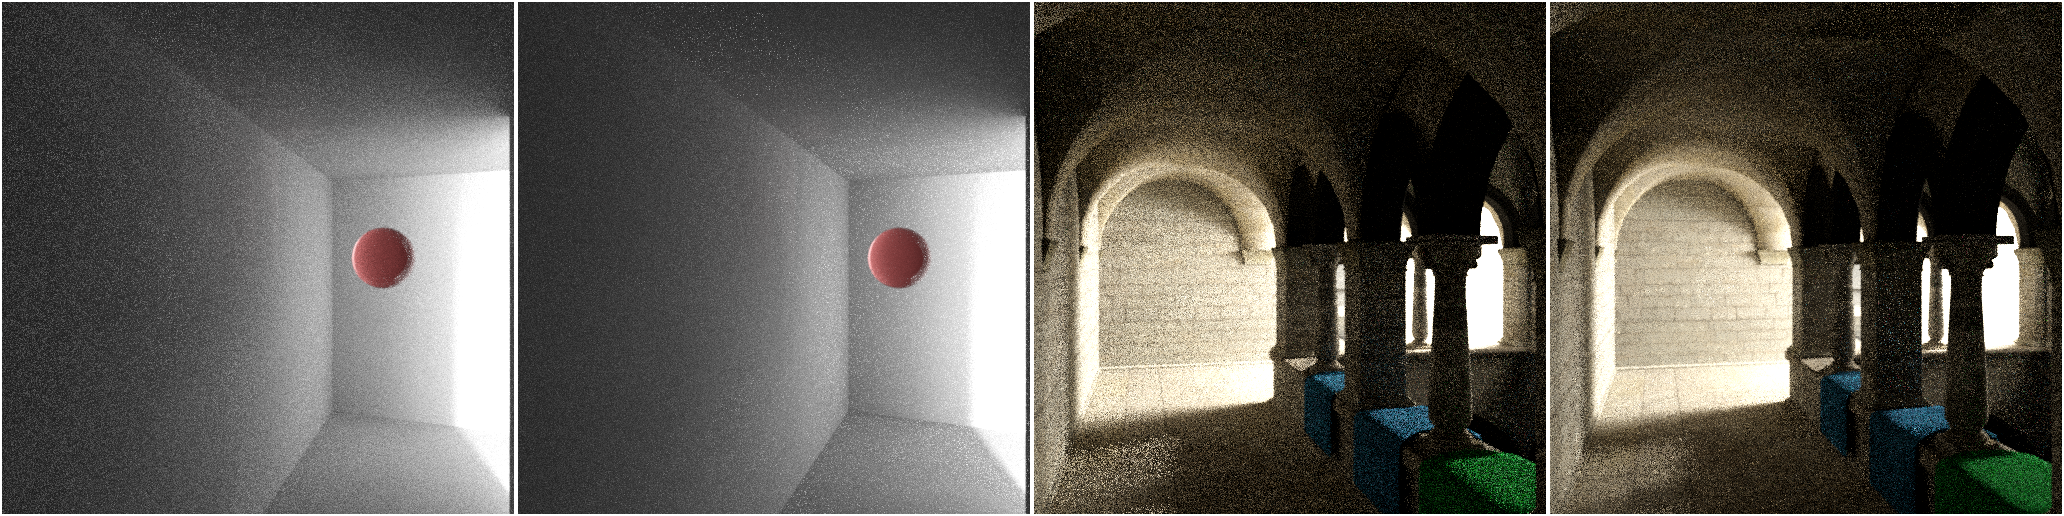
\includegraphics[scale=0.17]{images/four_scenes_for_dgci.png}
\caption{Four images comparing the classic path tracing (image $a$ and $c$) and our method (image $b$ and $d$). Note the noise reduction of our method in the left wall of images $a$ and $b$, and on the floor on image $c$ and $d$.}
\end{center}
\end{figure}

We observe that images produced by our algorithm have less noise than the ones produced by the regular path tracing (for a same number of rays shot per pixel). The MSE values are lower for the top pictures, meaning that we converge faster to the reference image than standard path tracing does.

This image is a zoom that allows us to see more precisely the the reduction of noise for our method.

\section{Conclusion}

We presented an application of our skeletonization algorithm for global illumination. Our strategy works well, it reduces noise by taking into account the distribution of energy in the scene. One of the problems is that we take into account only one importance direction for sampling, totally ignoring the BRDF and the cosine factor. A solution called Multiple Importance Sampling will allow us to combine different strategies into one.